\documentclass[preprint,12pt,authoryear]{elsarticle}

\usepackage[utf8]{inputenc}
\usepackage[T1]{fontenc}
\usepackage[margin=0.35in]{geometry}
\usepackage{graphicx}
\usepackage{amssymb}
\usepackage{amsmath}
\usepackage{booktabs}
\usepackage{siunitx}
\usepackage{xcolor}
\usepackage{float}
\usepackage{xurl}
\usepackage[hidelinks]{hyperref}

\graphicspath{{figures/}}
\renewcommand{\thefigure}{S\arabic{figure}}
\renewcommand{\thetable}{S\arabic{table}}

\begin{document}

\begin{frontmatter}

\title{Supplementary Information for: Existing Multi-Material FFF Printers Are Sufficient For (Near) Arbitrary Coloration}

\author{Anonymous author(s)}

\end{frontmatter}

\section*{Supplementary Methods}

\subsection*{Calibrated image acquisition and processing}

Printed gamut samples were photographed using a tripod-mounted Nikon Z5 full-frame mirrorless camera fitted with a NIKKOR Z MC 105~mm f/2.8 VR S macro lens. Samples were imaged in a diffuse LED light box under fixed illumination. The camera was operated manually at ISO~100, f/8, 1/40~s, and fixed daylight white balance. RAW NEF files were converted through a fixed color-correction workflow using an in-frame color calibration target. Color correction and white balance were applied before export as full-resolution 16-bit TIFF images. No subjective per-sample color edits were used for the analysis images.

Each triangular gamut image was analyzed independently. Filename labels defined the intended color anchors in bottom-left, top, and bottom-right order. The printed triangle was registered to the expected LayerLoom layout using manually checked landmarks. This manual check was important for low-contrast white and yellow vertices, where fully automatic contour fitting could place the triangle tip incorrectly. Benchy photographs were excluded from color-space measurement.

Expected regions were generated from the same palette-enumeration rules used to create the printed samples. Region colors were extracted from central-core masks rather than full polygons to reduce seam, border, shadow, and registration artifacts. Sampled pixels were converted to CIE \(L^*a^*b^*\), trimmed by excluding outliers beyond the 98th percentile of distance from the region median, and summarized by median \(L^*a^*b^*\) and RGB values. Distinguishable-color counts were estimated by connecting measured regions with pairwise \(\Delta E_{00}\) below the stated threshold and counting connected components. Hull area was computed from measured CIE \(a^*b^*\) coordinates.

\subsection*{Filaments used for printed color endpoints}

Printed color samples used commercially available PLA filaments. Bambu Lab endpoint colors were PLA Basic unless otherwise noted. Exact catalog names or SKUs were not recorded for every Bambu Lab color endpoint, so supplier and color descriptions are reported as used during printing. The non-Bambu endpoint filaments were Printed Solid Jessie PLA orange and OVERTURE PLA purple. In the expanded-gamut analysis, \(L\) denotes the Bambu Lab light-gray endpoint, \(N\) denotes the darker neutral-gray endpoint, and \(G\) denotes green.

\subsection*{Benchmark measurements}

Nine-cube benchmark plates used a 3-by-3 arrangement of 15~mm cubes with a 3~mm gap. Prints were sliced at 0.12~mm layer height with a 0.24~mm first layer. Snapmaker U1 and Bambu Lab X1C values in the final benchmark table are physical measurements of elapsed print time and material use. Prusa XL values are slicer estimates, retained as a multi-toolhead reference because physical Prusa XL prints were not available for the final measured set.

\subsection*{Supplementary data files}

The figure directory contains rendered supplementary figures. The accompanying \texttt{tables/} directory contains CSV summaries for condition-level color measurements, distinguishability thresholds, theoretical recipe counts, duplicate repeatability, benchmark values, filament endpoints, and Benchy gallery membership. Numerical values used in the supplementary tables are written directly into this document and mirrored in the CSV files for reproducibility.

\section*{Supplementary Tables}

\begin{table}[H]
\centering
\caption{\textbf{Theoretical layer-fraction recipe counts for endpoint alphabets used in the expanded-gamut analysis.}
Counts collapse redundant stack orderings with identical layer fractions. These values describe enumerated design spaces for the listed alphabets, not the number of experimentally distinguishable printed colors or the number of colors used in any single printed triangular gamut.}
\small
\begin{tabular}{llrrrr}
\toprule
Condition & Palette family & Alphabet & Recipes & \(H_{\max}\) & Run limit \\
\midrule
Two-color & CMY & cmy & 30 & 6 & 2 \\
Two-color & CMY+neutral & cmykwnl & 196 & 6 & 2 \\
Two-color & CMY+OVG & cmyovg & 141 & 6 & 2 \\
Two-color & CMY+neutral+OVG & cmykwnlovg & 415 & 6 & 2 \\
Full & CMY & cmy & 55 & 6 & 5 \\
Full & CMY+neutral & cmykwnl & 1554 & 6 & 5 \\
Full & CMY+OVG & cmyovg & 812 & 6 & 5 \\
Full & CMY+neutral+OVG & cmykwnlovg & 7447 & 6 & 5 \\
\bottomrule
\end{tabular}
\label{tab:supp-theoretical-counts}
\end{table}

\begin{table}[H]
\centering
\caption{\textbf{Measured color coverage summaries.}
Measured regions are printed region observations across the corresponding endpoint-substitution gamut samples. Distinguishable counts are connected-component counts after thresholding pairwise CIEDE2000 distances.}
\scriptsize
\setlength{\tabcolsep}{4pt}
\begin{tabular}{llrrrrr}
\toprule
Condition & Palette family & Regions & \(\Delta E_{00}<2\) & \(\Delta E_{00}<5\) & Hull area & Median NN \(a^*b^*\) \\
\midrule
Two-color & CMY & 30 & 30 & 12 & 6226 & 13.76 \\
Two-color & CMY+OVG & 270 & 69 & 13 & 8346 & 4.43 \\
Two-color & CMY+neutral & 360 & 98 & 11 & 5768 & 4.00 \\
Two-color & CMY+neutral+OVG & 660 & 161 & 17 & 8626 & 2.98 \\
Full & CMY & 55 & 51 & 23 & 6646 & 6.48 \\
Full & CMY+OVG & 495 & 152 & 9 & 8146 & 2.42 \\
Full & CMY+neutral & 660 & 298 & 28 & 7042 & 1.97 \\
Full & CMY+neutral+OVG & 1210 & 393 & 22 & 8752 & 1.57 \\
\bottomrule
\end{tabular}
\label{tab:supp-color-summary}
\end{table}

\begin{table}[H]
\centering
\caption{\textbf{Nine-cube benchmark values.}
Bambu X1C and Snapmaker U1 values are measured. Prusa XL values are slicer estimates.}
\small
\begin{tabular}{llrrrrr}
\toprule
Printer & Metric & A1 & A2 & A3 & A4 & A5 \\
\midrule
Bambu X1C & Time (min) & 330 & 324 & 360 & 600 & 609 \\
Bambu X1C & Material/waste (g) & 85.45 & 86.12 & 85.46 & 157.86 & 155.25 \\
Snapmaker U1 & Time (min) & 103 & 103 & 104 & 133 & 133 \\
Snapmaker U1 & Material (g) & 20.10 & 20.48 & 20.37 & 24.81 & 24.80 \\
Prusa XL & Time estimate (min) & 186 & 185 & 185 & 217 & 217 \\
Prusa XL & Material estimate (g) & 24.13 & 24.12 & 24.12 & 28.30 & 28.30 \\
\bottomrule
\end{tabular}
\label{tab:supp-benchmark-values}
\end{table}

\begin{table}[H]
\centering
\caption{\textbf{Repeatability checks for calibrated photographic measurements.}
Duplicate photographs of the same printed gamut were independently processed and compared region by region. Values shown are CIEDE2000 distances between duplicate measurements.}
\scriptsize
\setlength{\tabcolsep}{2pt}
\begin{tabular}{@{}p{0.15\linewidth}p{0.34\linewidth}p{0.08\linewidth}p{0.12\linewidth}p{0.13\linewidth}p{0.10\linewidth}@{}}
\toprule
Condition & Duplicate pair & Regions & Median \(\Delta E_{00}\) & 95th percentile & Maximum \\
\midrule
Two-color CMY & \texttt{cmysimpleDSC\_4511} vs \texttt{cmysimpleDSC\_4512} & 30 & 0.24 & 0.77 & 1.09 \\
Full YWM & \texttt{DSC\_4523ywm} vs \texttt{DSC\_4524ywm} & 55 & 0.20 & 0.95 & 1.20 \\
\bottomrule
\end{tabular}
\label{tab:supp-repeatability}
\end{table}

\begin{table}[H]
\centering
\caption{\textbf{Filaments used for printed color endpoints.}
All entries are commercially available PLA filaments. Bambu Lab entries were PLA Basic unless otherwise noted. Exact catalog names or SKUs were not recorded for every Bambu Lab endpoint color.}
\scriptsize
\setlength{\tabcolsep}{3pt}
\begin{tabular}{p{0.06\linewidth}p{0.13\linewidth}p{0.35\linewidth}p{0.36\linewidth}}
\toprule
Token & Endpoint & Filament/source & Notes \\
\midrule
C & Cyan & Bambu Lab PLA Basic cyan endpoint & Exact catalog color name not recorded. \\
M & Magenta & Bambu Lab PLA Basic magenta/pink endpoint & Exact catalog color name not recorded. \\
Y & Yellow & Bambu Lab PLA Basic yellow endpoint & Exact catalog color name not recorded. \\
W & White & Bambu Lab PLA Basic white endpoint & Exact catalog color name not recorded. \\
L & Light gray & Bambu Lab PLA Basic light gray & Used as the light-gray endpoint in expanded-gamut photo analysis. \\
N & Dark neutral gray & Bambu Lab PLA Basic Gray (10103), refill, 1~kg & Used as the darker neutral-gray endpoint in expanded-gamut photo analysis. \\
K & Black & Bambu Lab PLA Basic black & Used as the black/value endpoint. \\
O & Orange & Printed Solid Jessie PLA orange & Used as the orange expanded-gamut endpoint. \\
V & Violet/purple & OVERTURE PLA purple, 1.75~mm, 1~kg spool, \(\pm 0.02\)~mm dimensional accuracy & Used as the violet/purple expanded-gamut endpoint. \\
G & Green & Bambu Lab PLA Basic green endpoint & Exact catalog color name not recorded. \\
\bottomrule
\end{tabular}
\label{tab:supp-filaments}
\end{table}

\clearpage
\section*{Supplementary Figures}

\begin{figure}[p]
    \centering
    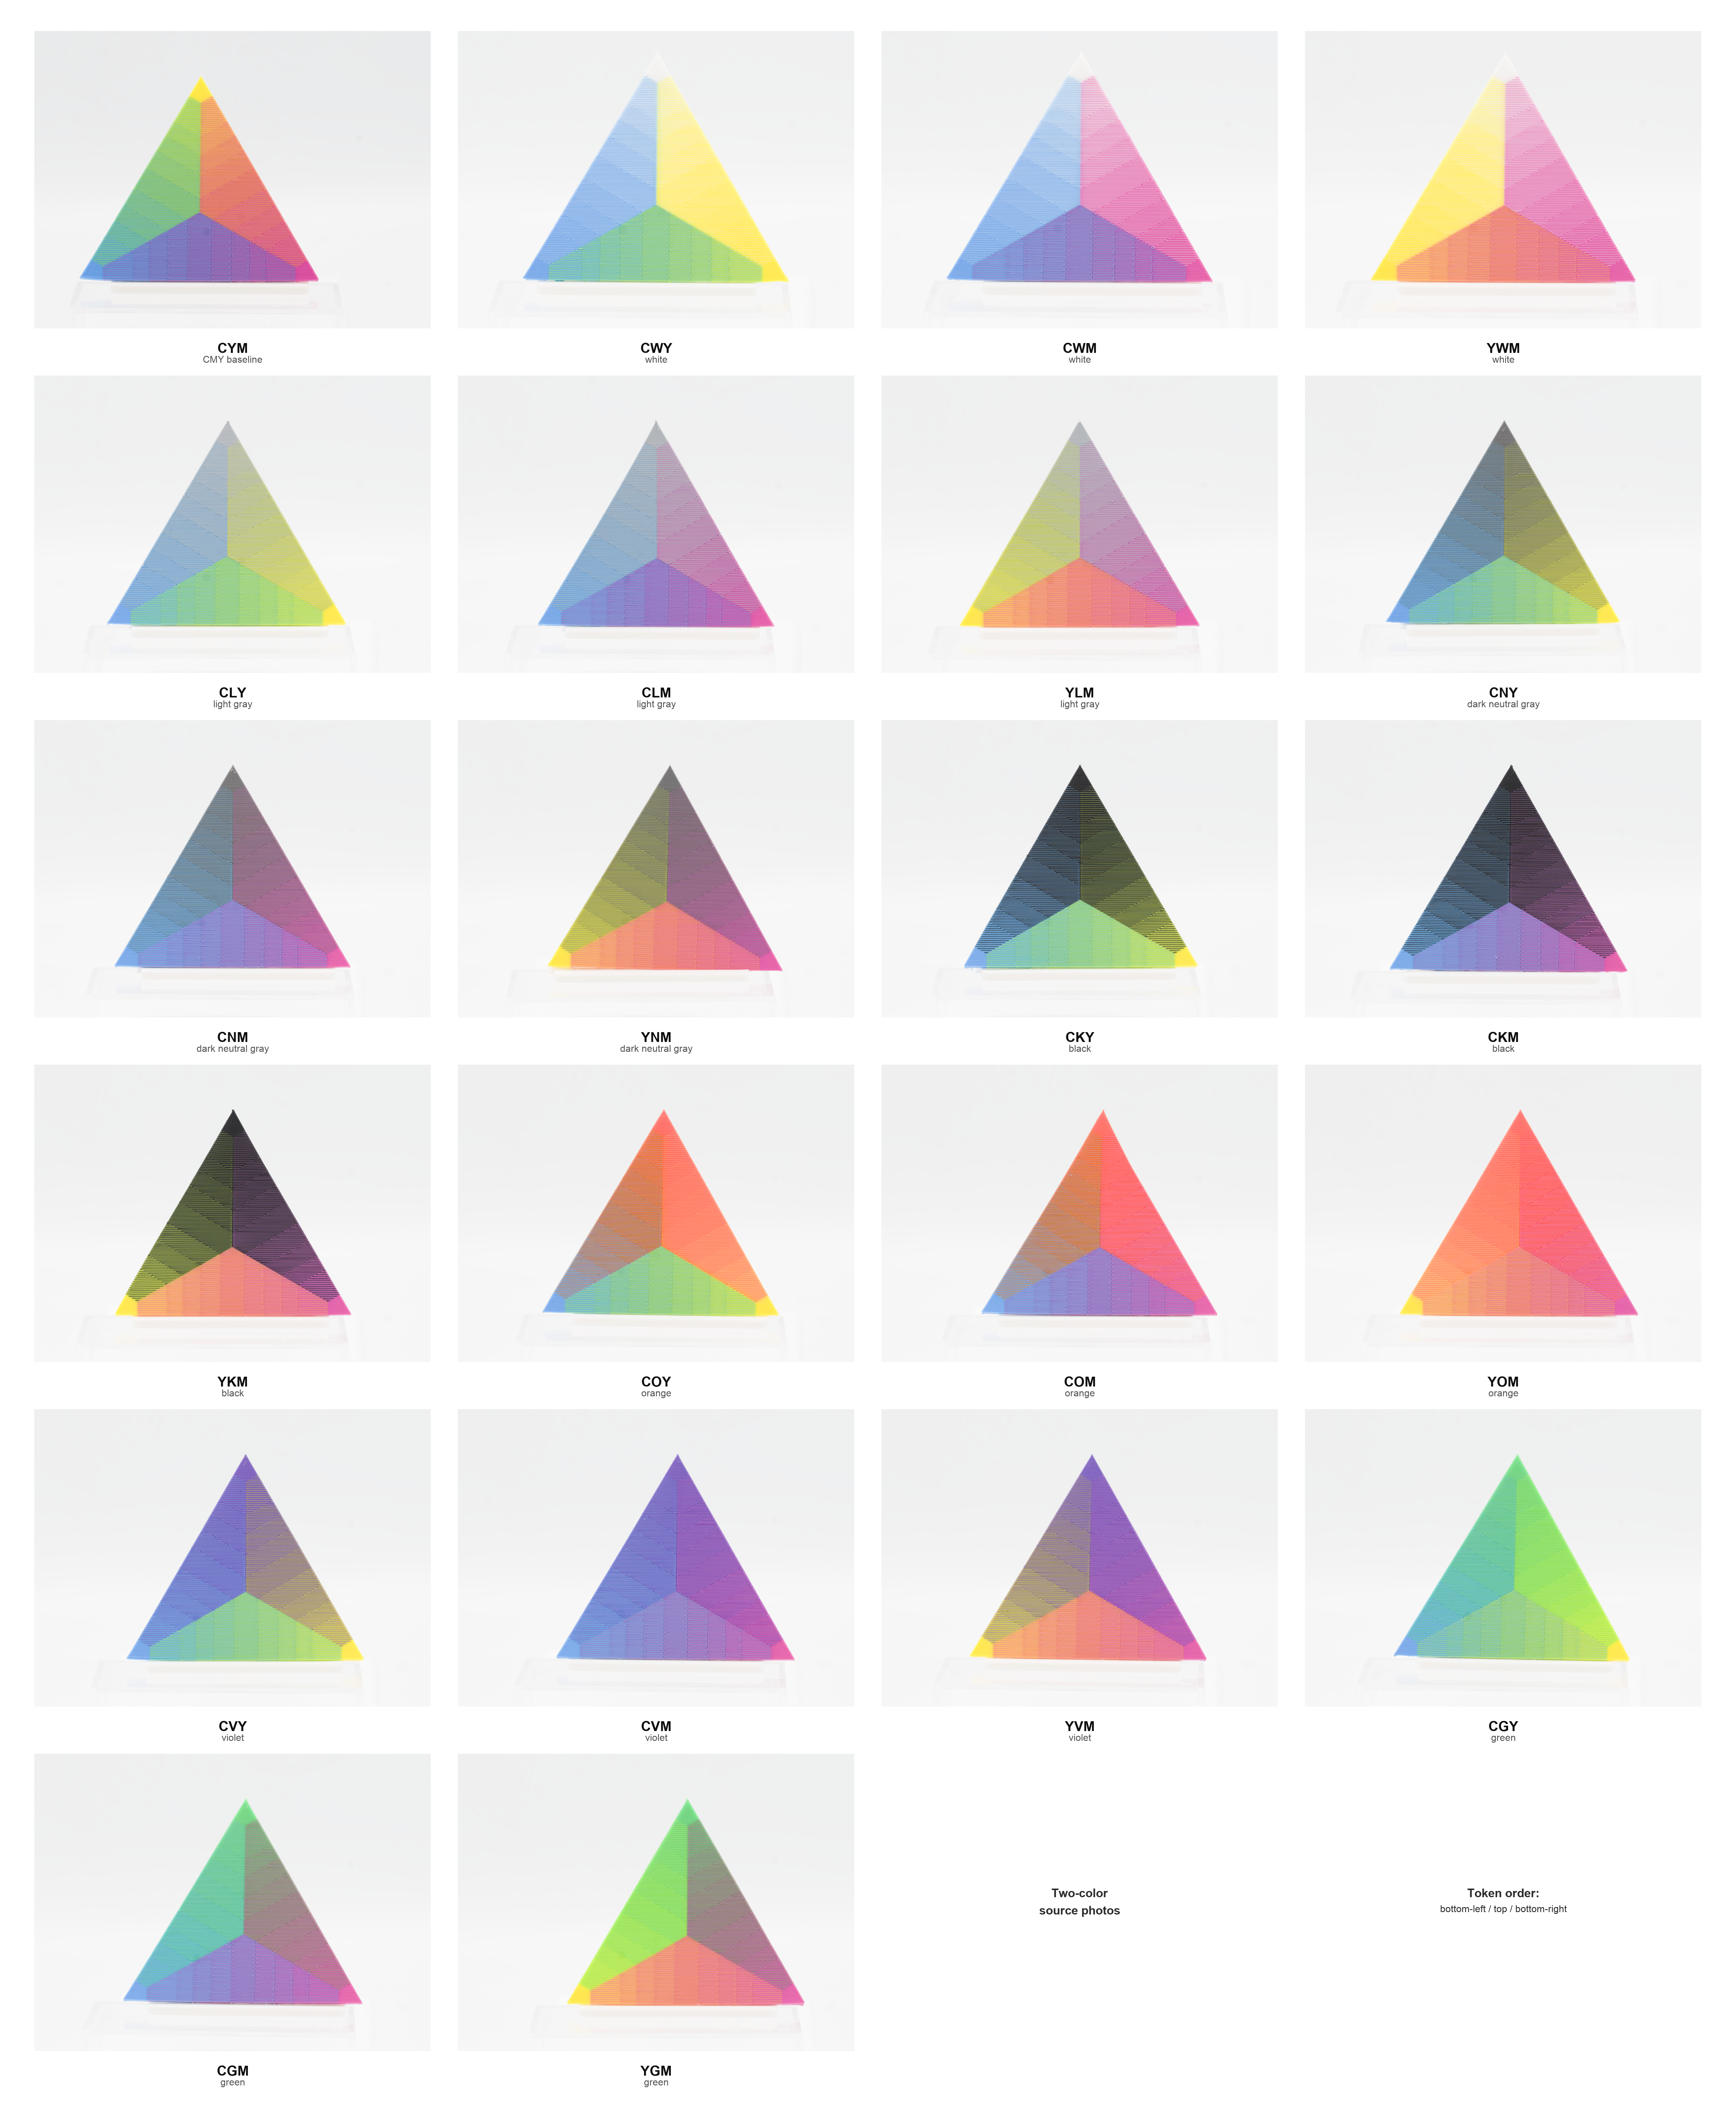
\includegraphics[width=\textwidth,height=0.88\textheight,keepaspectratio]{supp_fig01_two_color_triangle_photo_gallery.png}
    \caption{\textbf{Supplementary Figure S1. Two-color expanded endpoint source photographs.}
    Calibrated source photographs for the two-color triangular gamut samples used in expanded endpoint analysis. Each tile shows one printed triangular gamut before region extraction. Token labels indicate the endpoint order as bottom-left, top, and bottom-right.}
    \label{fig:supp-two-color-source-photos}
\end{figure}

\begin{figure}[p]
    \centering
    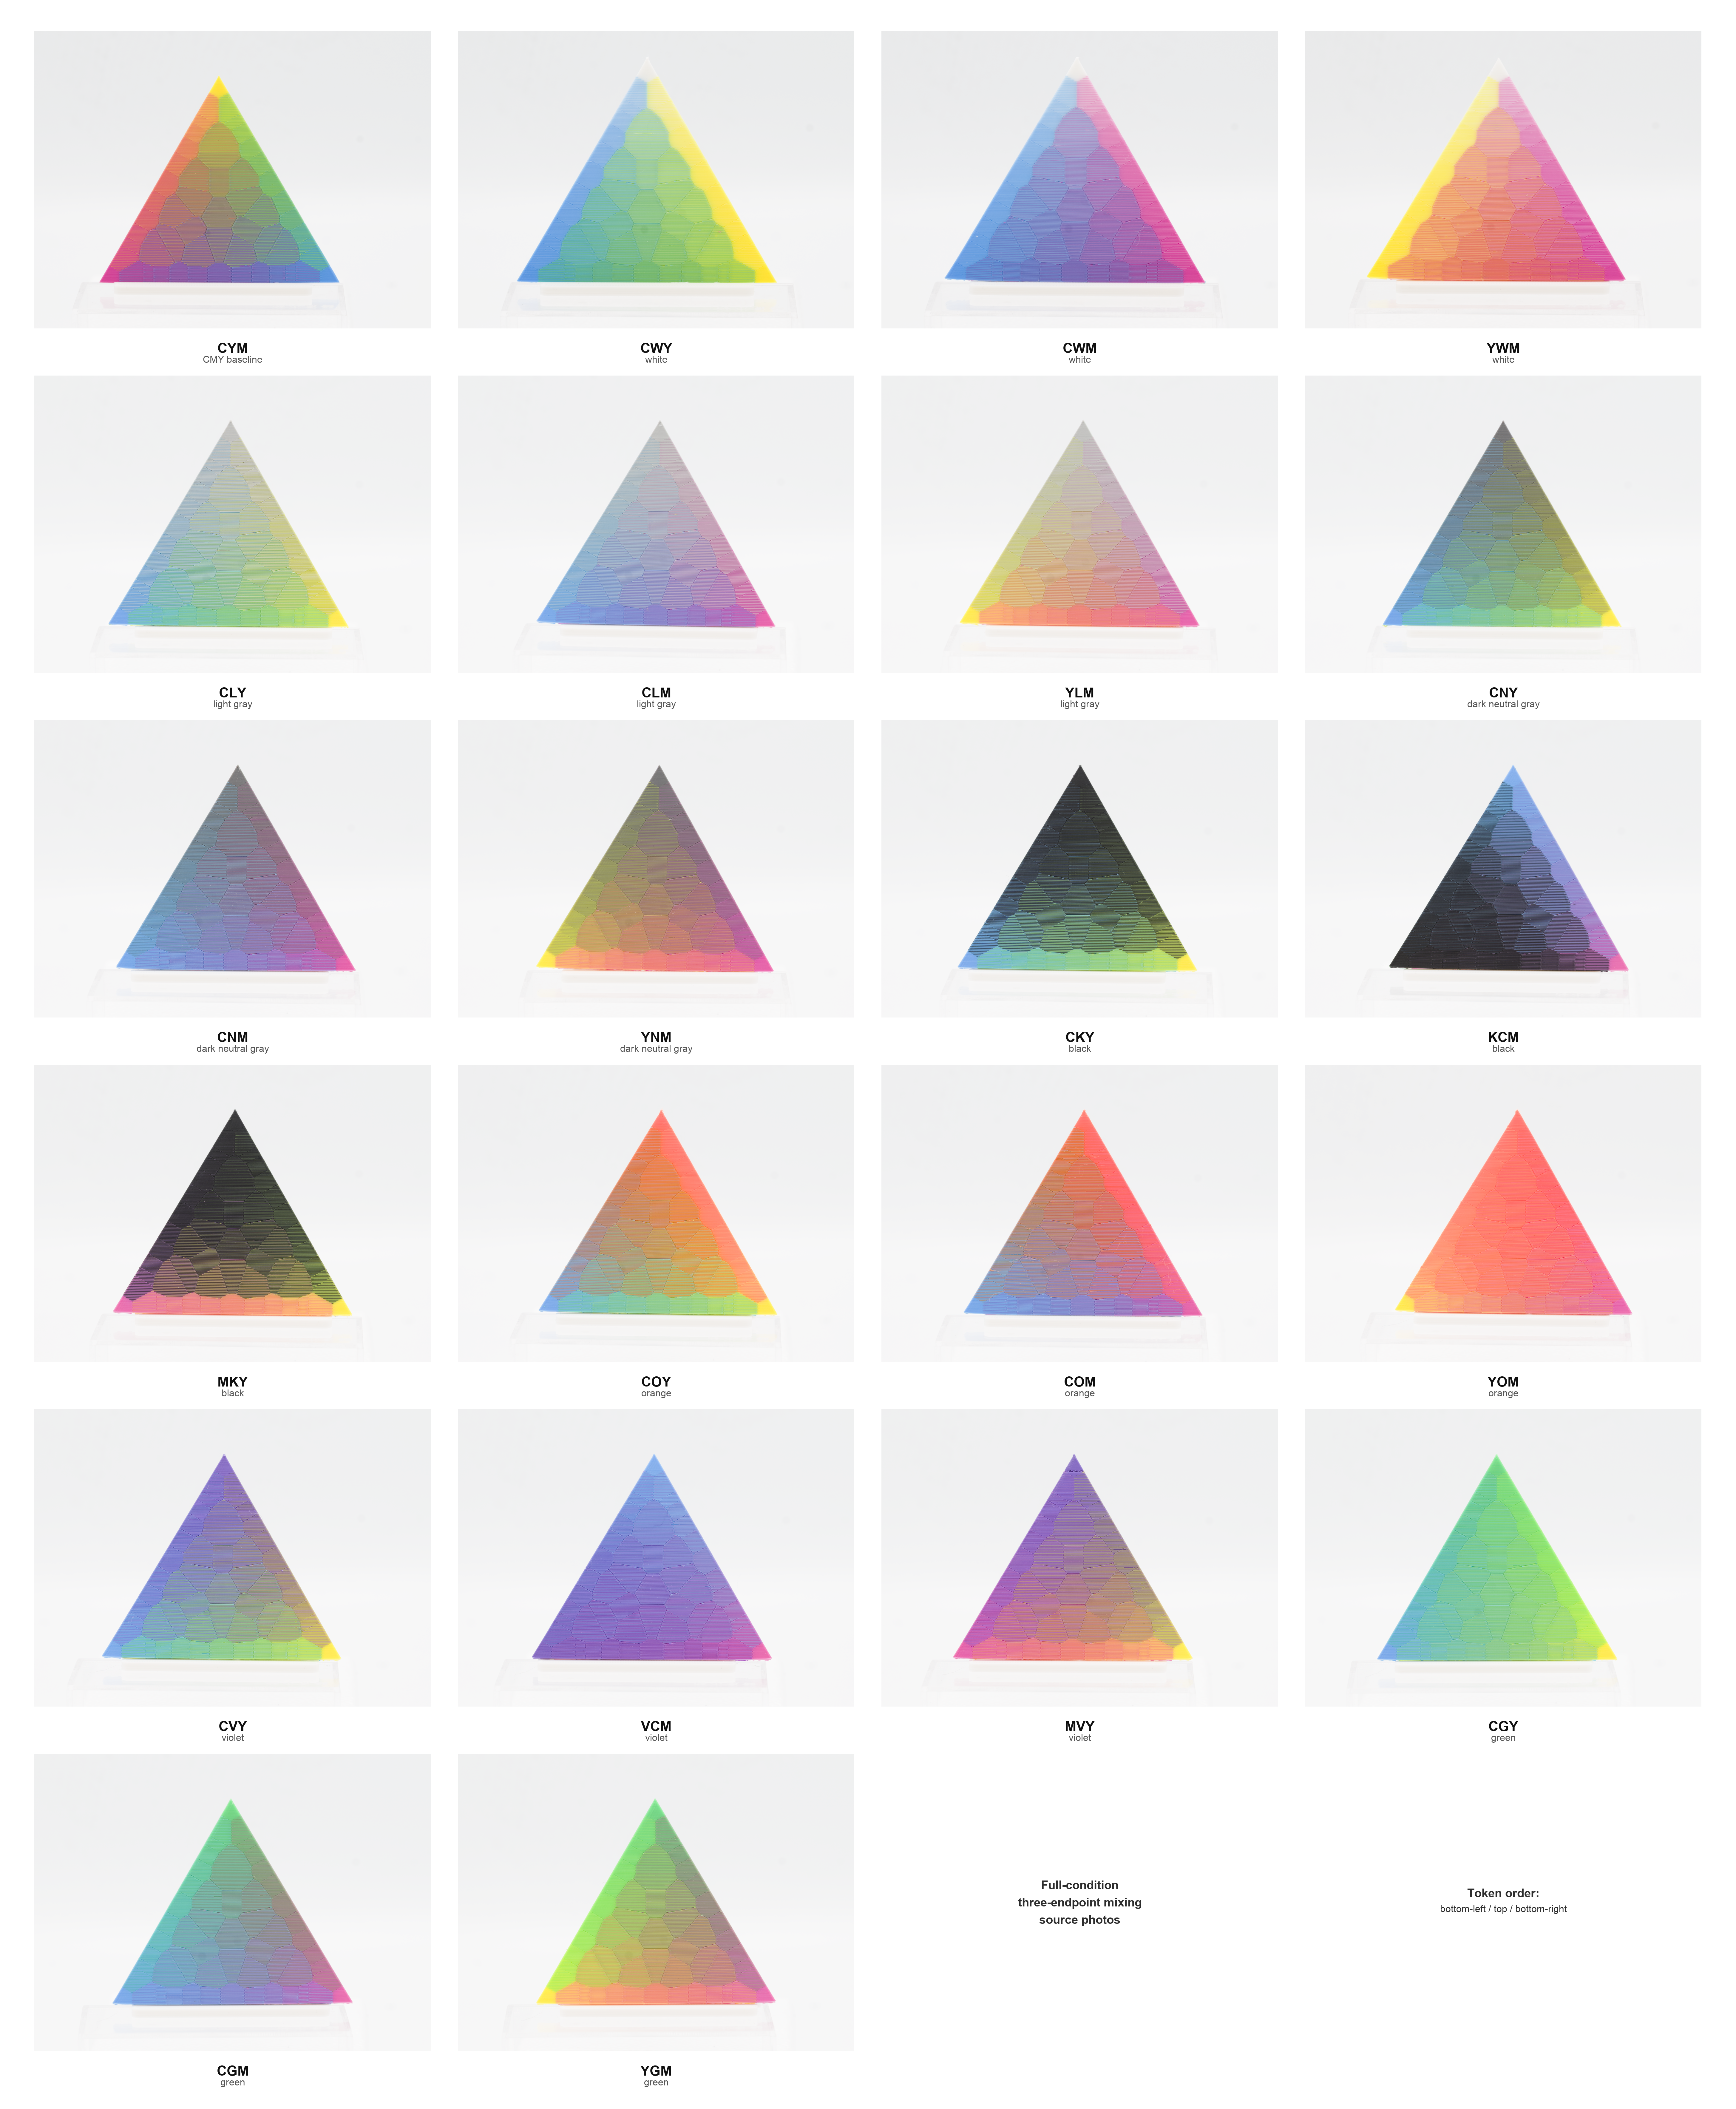
\includegraphics[width=\textwidth,height=0.88\textheight,keepaspectratio]{supp_fig02_full_triangle_photo_gallery.png}
    \caption{\textbf{Supplementary Figure S2. Full-condition expanded endpoint source photographs.}
    Calibrated source photographs for the full-condition triangular gamut samples. These samples include three-endpoint mixing within each triangle and provide the source photographs for the expanded full-condition color-coverage measurements. Token labels indicate the endpoint order as bottom-left, top, and bottom-right.}
    \label{fig:supp-full-source-photos}
\end{figure}

\begin{figure}[p]
    \centering
    
\includegraphics[width=\textwidth,height=0.88\textheight,keepaspectratio]{supp_fig03_full_expanded_endpoint_mosaics.png}
    \caption{\textbf{Supplementary Figure S3. Full-condition expanded endpoint source mosaics.}
    Full-condition triangular endpoint substitutions used for expanded color-coverage measurements.}
    \label{fig:supp-full-mosaics}
\end{figure}

\begin{figure}[p]
    \centering
    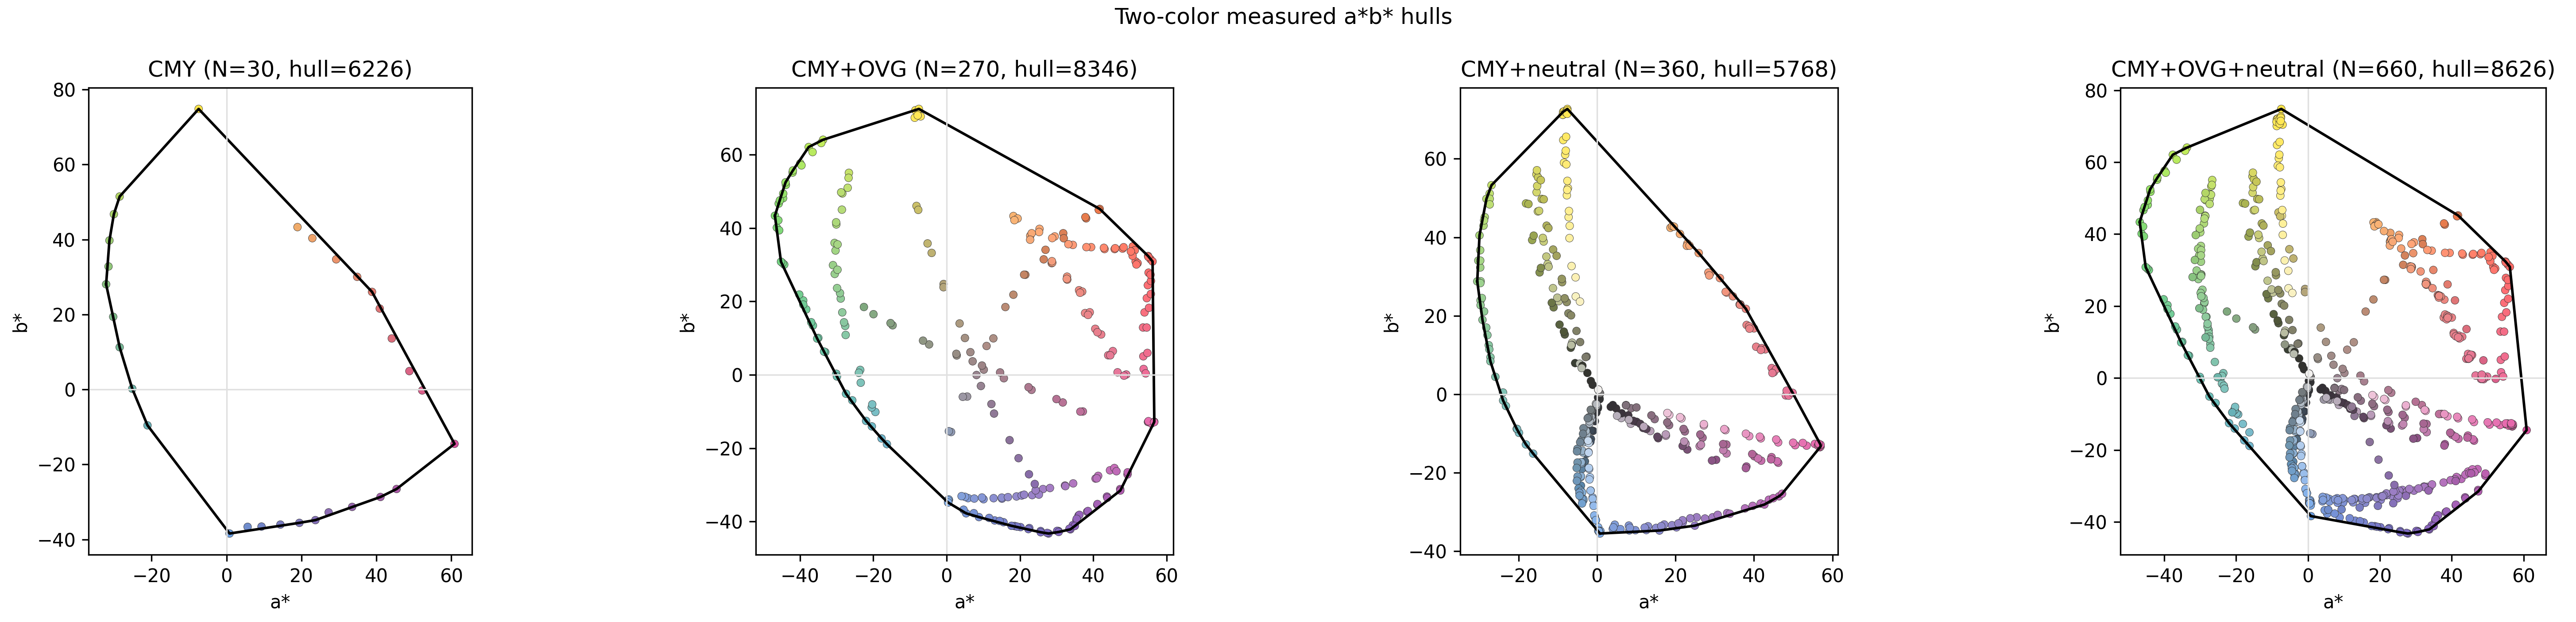
\includegraphics[width=\textwidth,height=0.88\textheight,keepaspectratio]{supp_fig04_two_color_measured_hulls.png}
    \caption{\textbf{Supplementary Figure S4. Two-color measured CIE \(a^*b^*\) hulls.}
    Measured median region colors and convex hulls for two-color CMY, CMY+OVG, CMY+neutral, and combined endpoint sets.}
    \label{fig:supp-two-color-hulls}
\end{figure}

\begin{figure}[p]
    \centering
    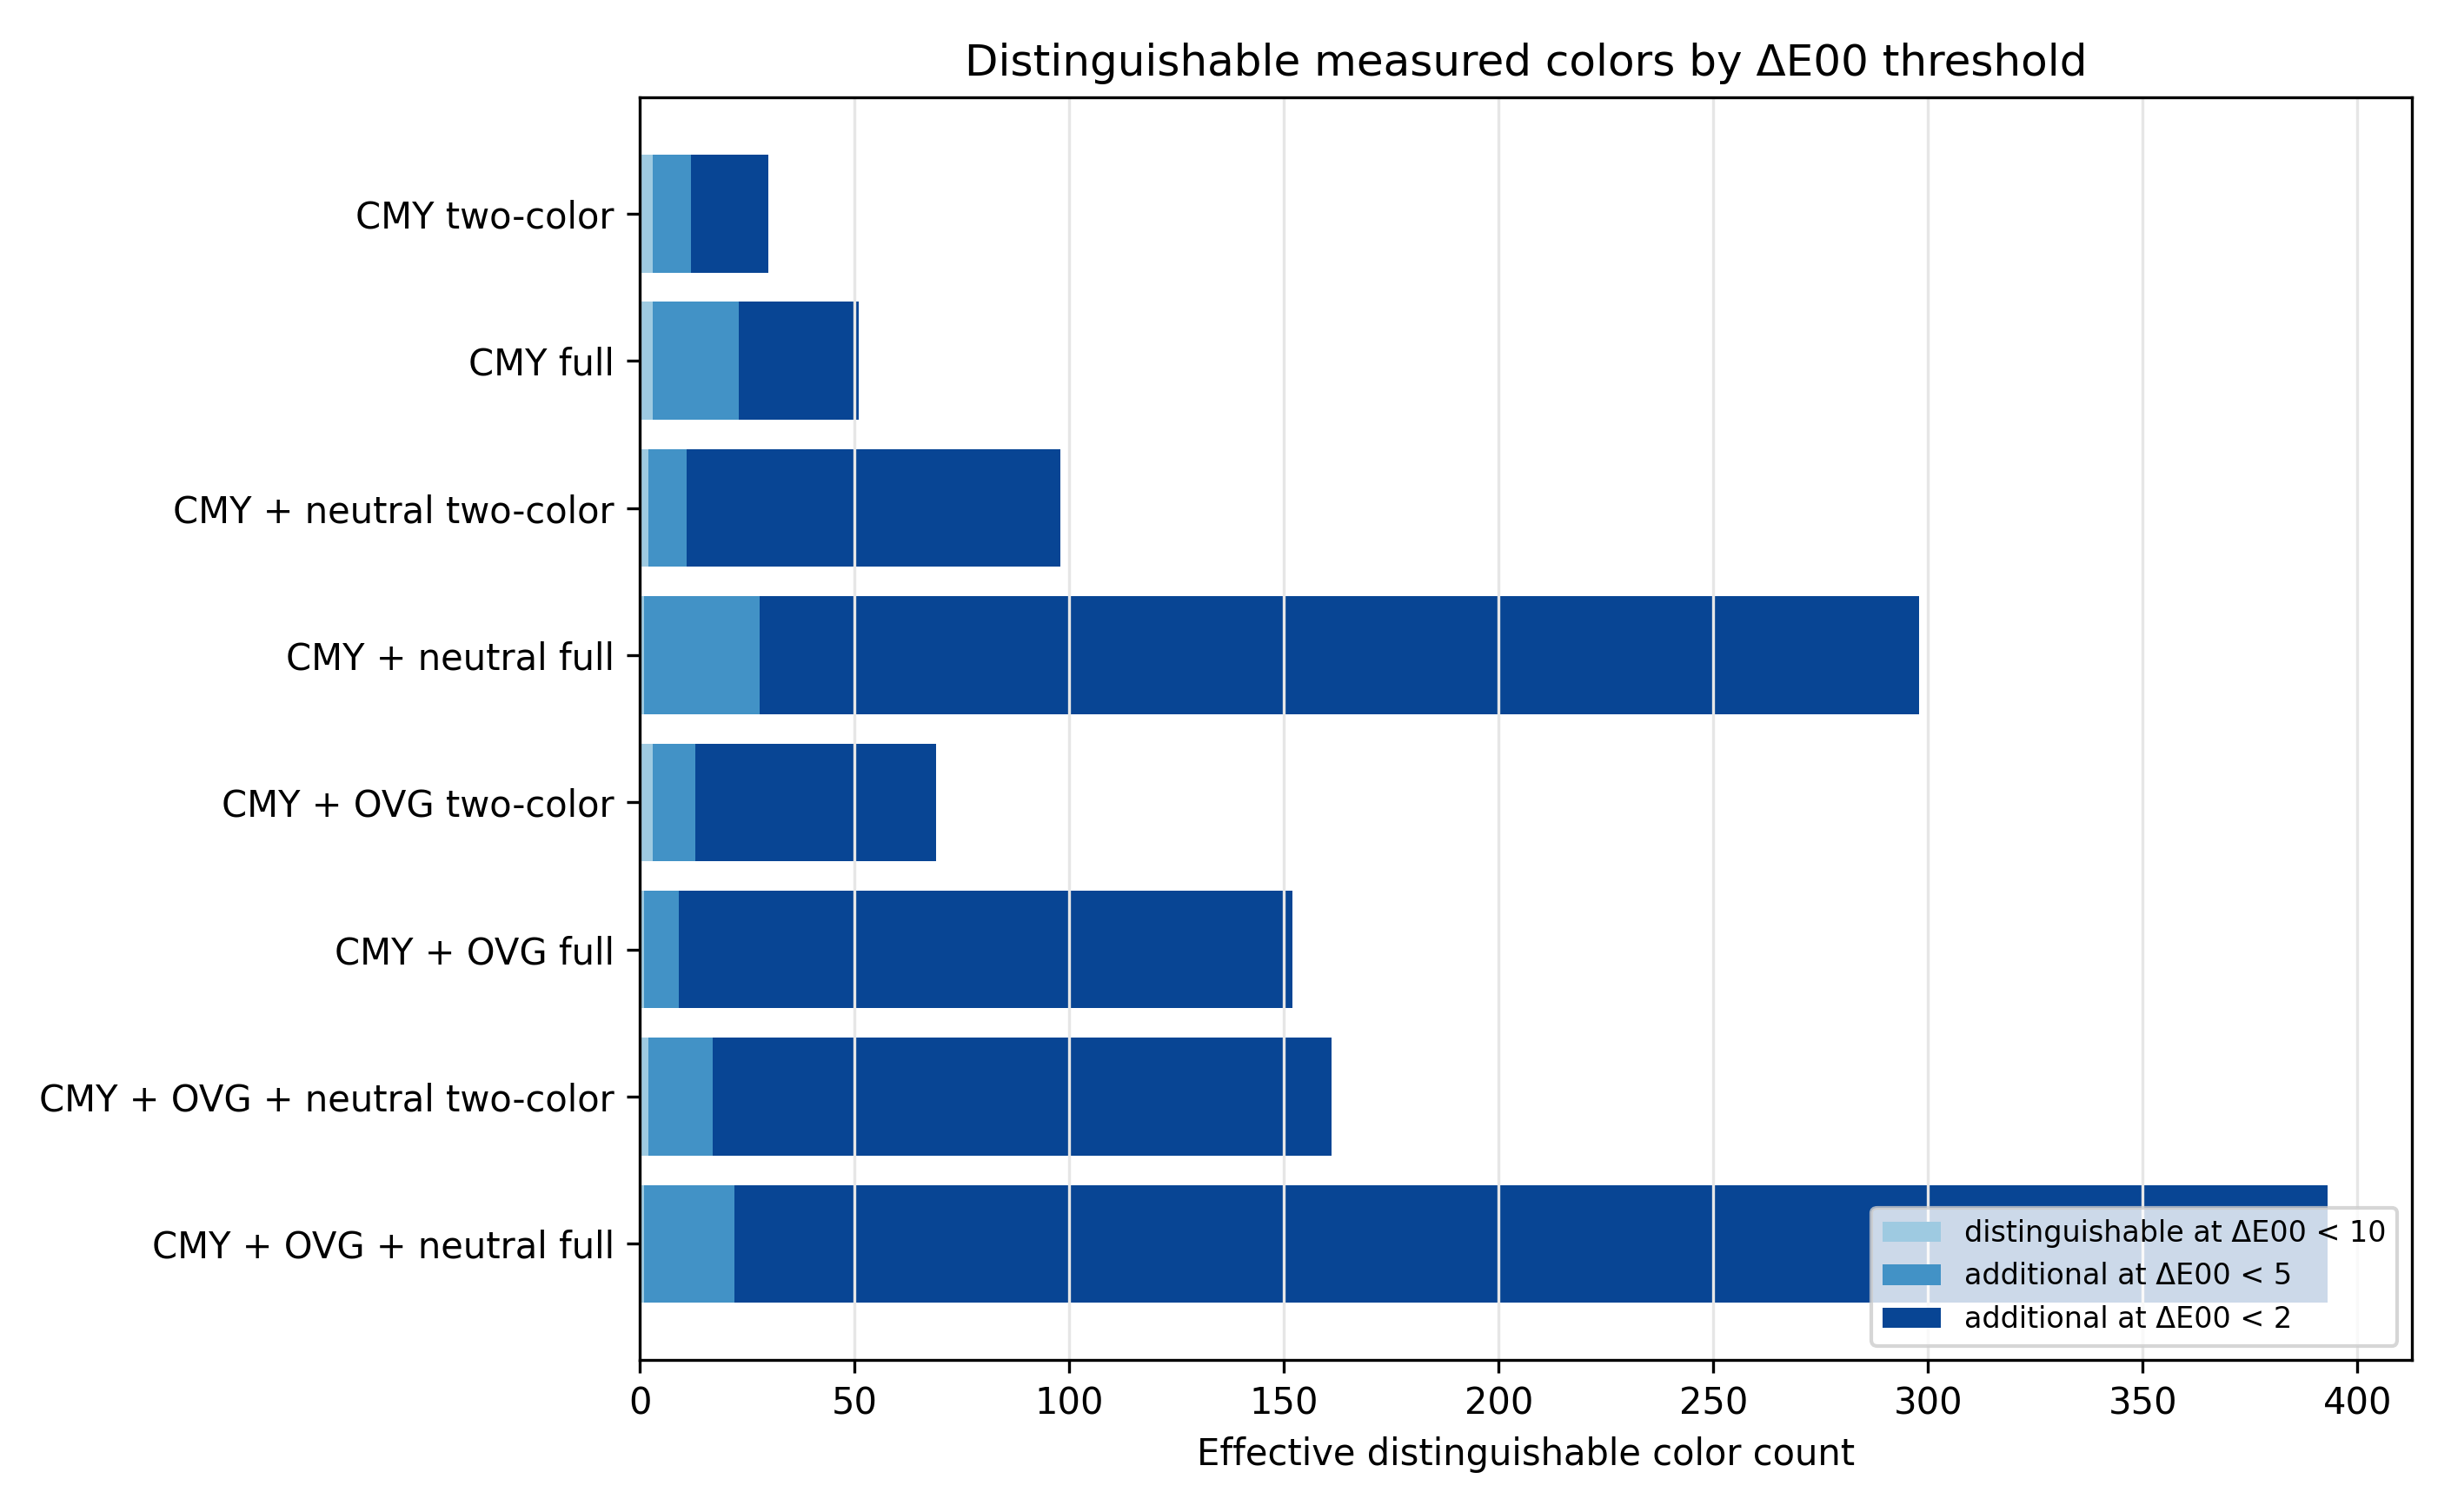
\includegraphics[width=\textwidth,height=0.88\textheight,keepaspectratio]{supp_fig05_distinguishable_color_counts.png}
    \caption{\textbf{Supplementary Figure S5. Distinguishable-color counts across thresholds.}
    Effective color-state counts at \(\Delta E_{00}<2\), \(<5\), and \(<10\), estimated from connected components of thresholded pairwise color distances.}
    \label{fig:supp-distinguishable-counts}
\end{figure}

\begin{figure}[p]
    \centering
    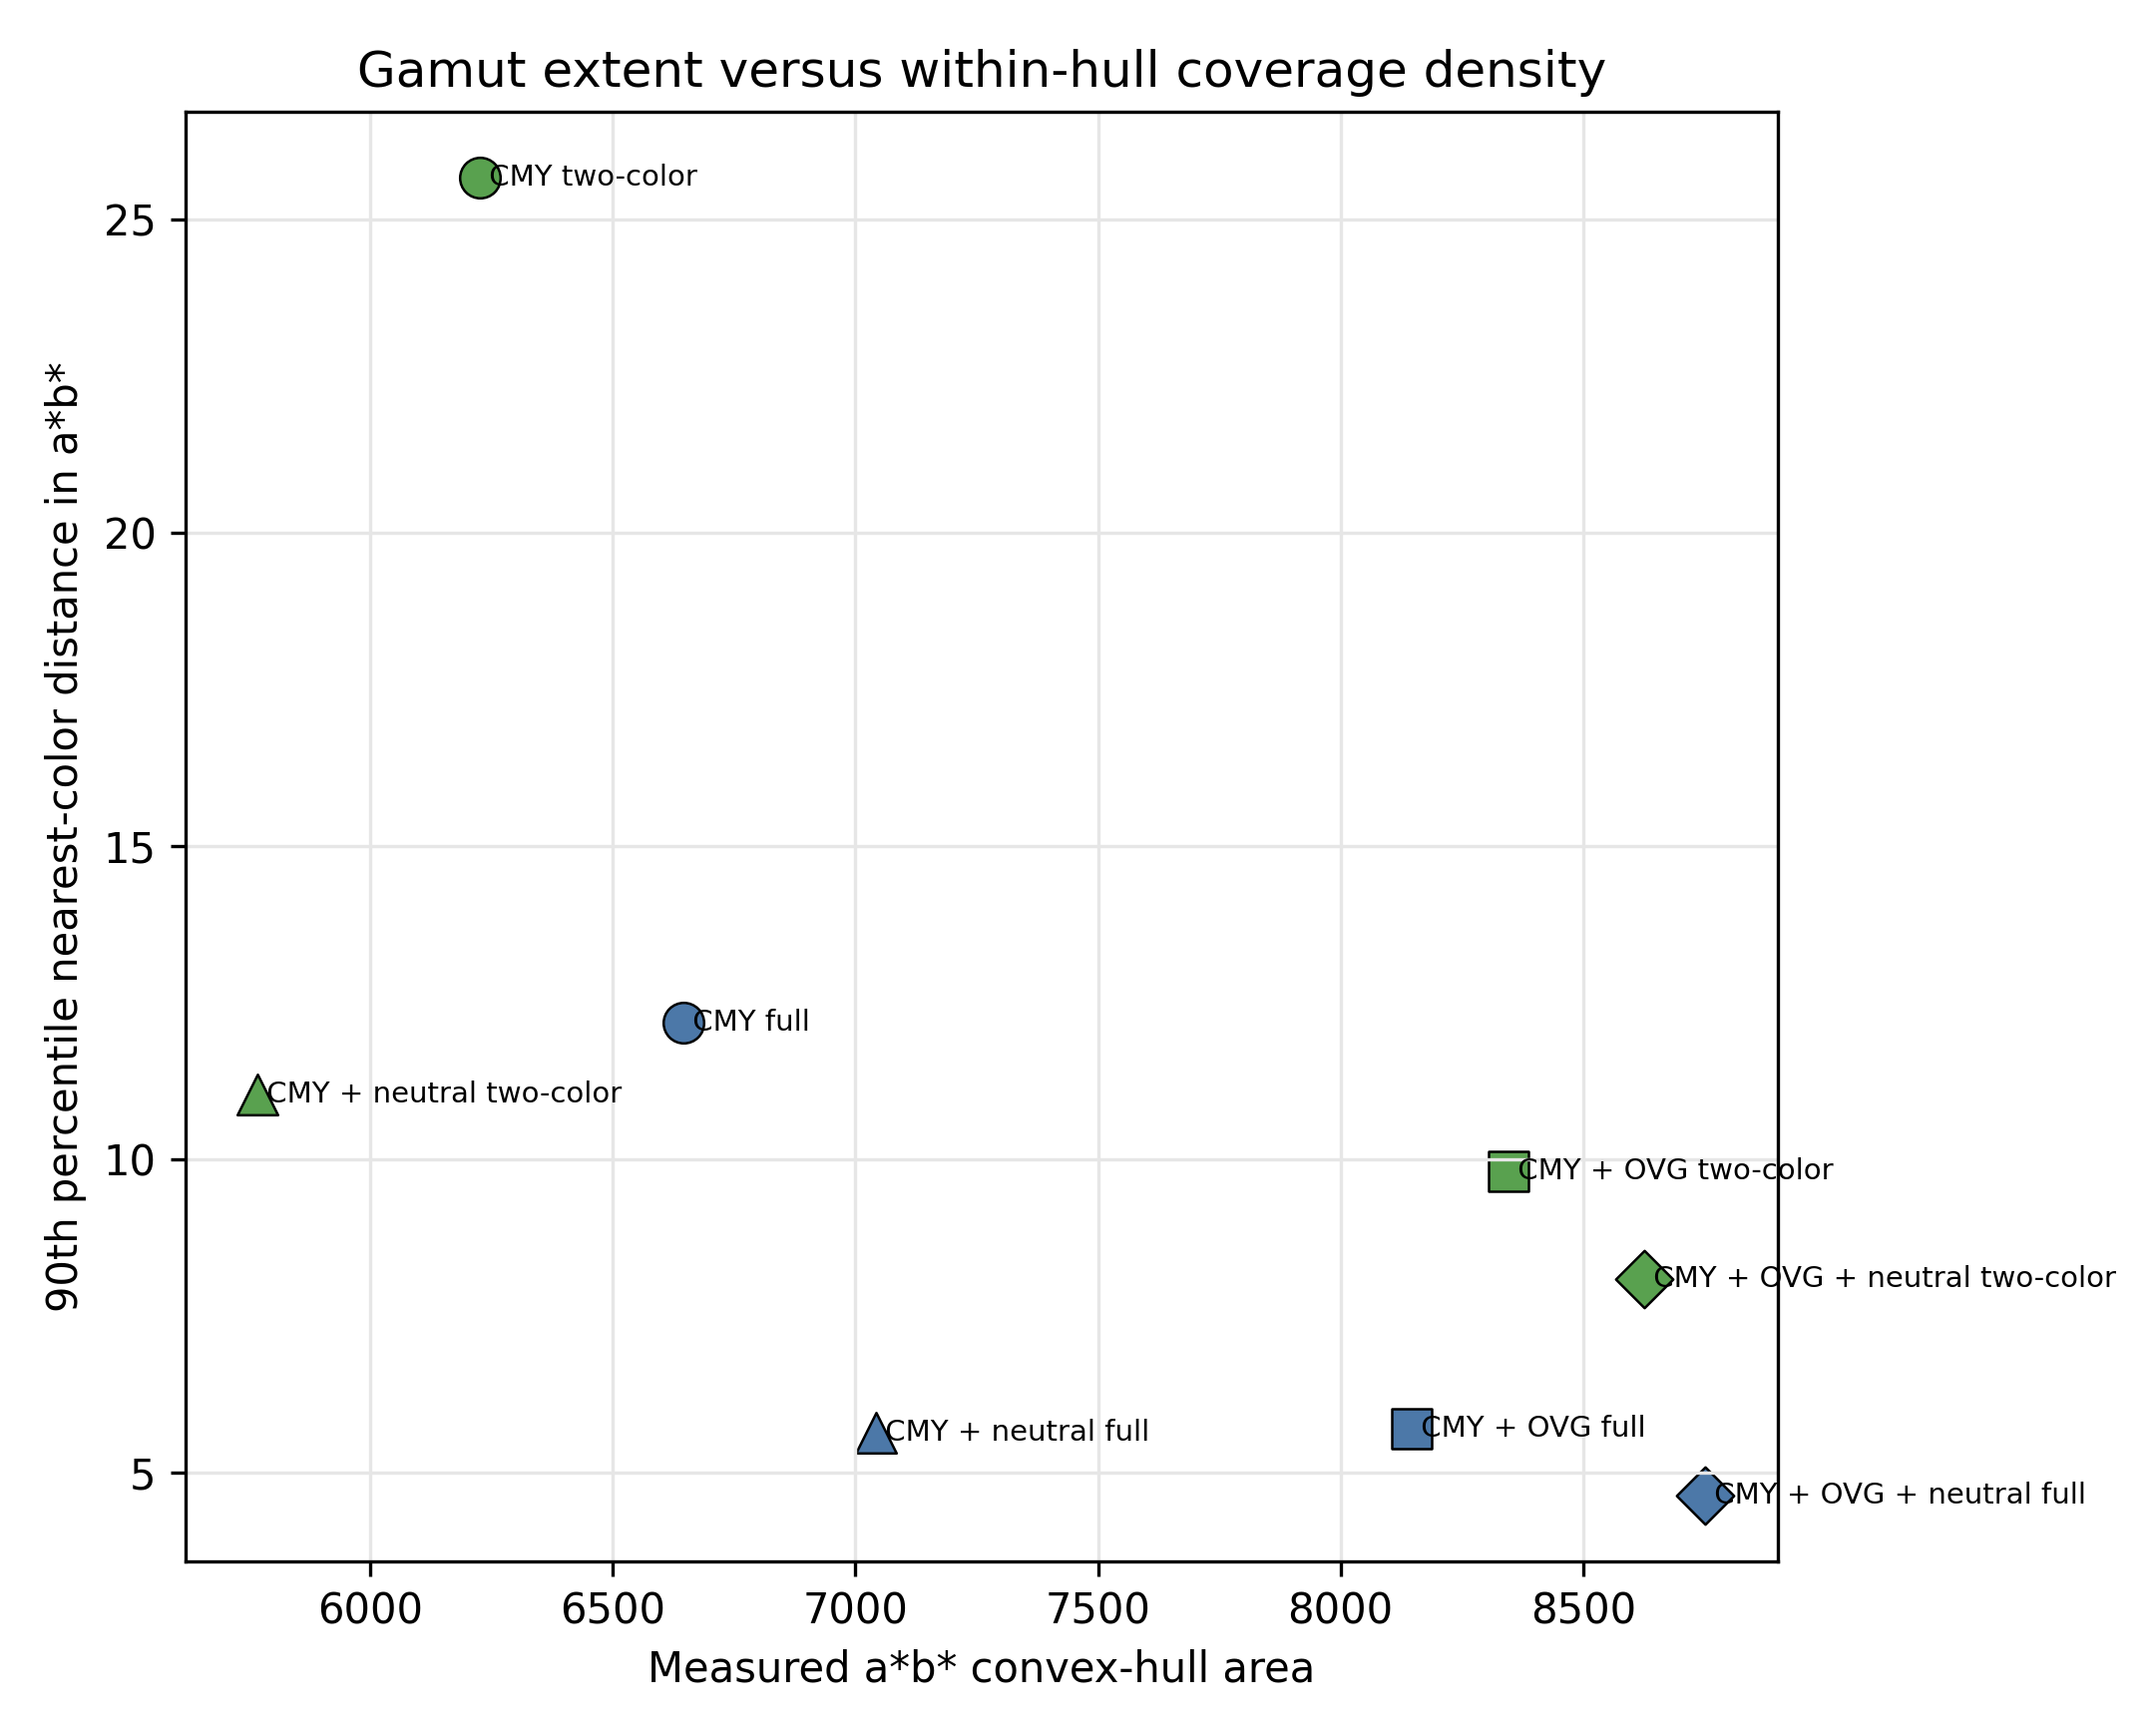
\includegraphics[width=\textwidth,height=0.88\textheight,keepaspectratio]{supp_fig06_hull_area_and_density.png}
    \caption{\textbf{Supplementary Figure S6. Coverage and density summaries.}
    Convex-hull area estimates chromatic extent, while the density metric summarizes spacing among measured colors within the hull.}
    \label{fig:supp-coverage-density}
\end{figure}

\begin{figure}[p]
    \centering
    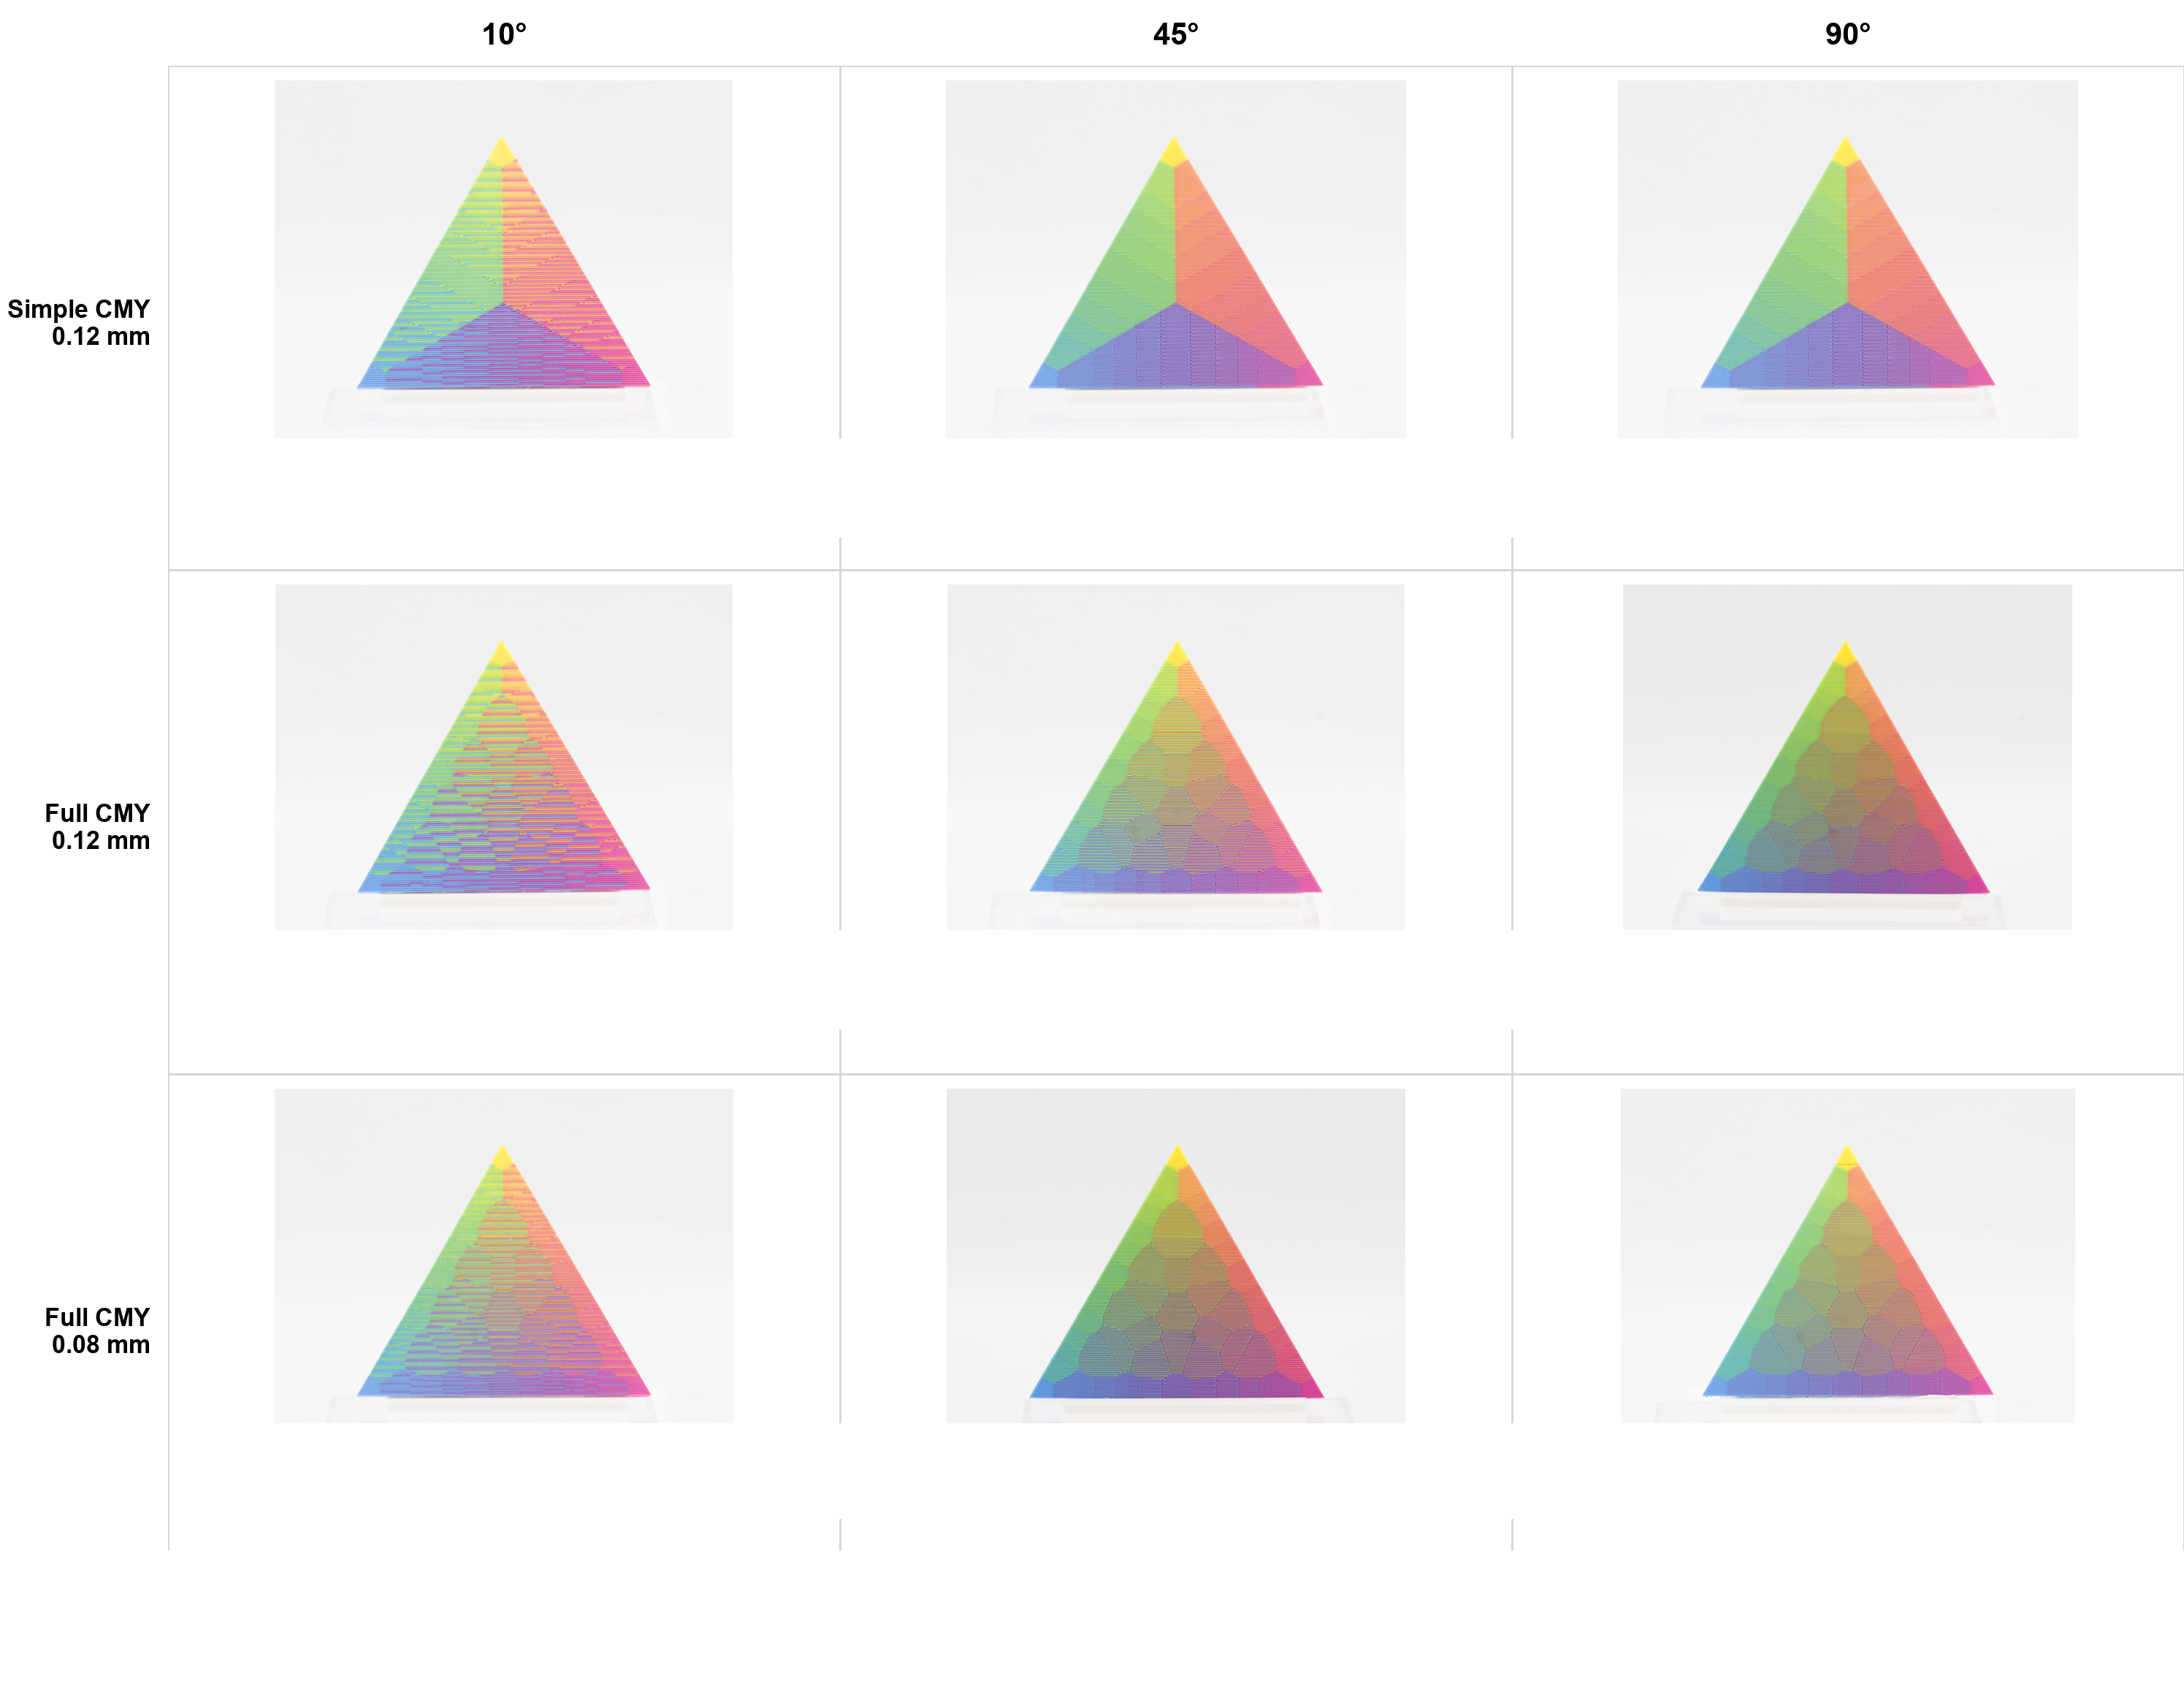
\includegraphics[width=\textwidth,height=0.88\textheight,keepaspectratio]{supp_fig07_orientation_angle_gamut_sources.png}
    \caption{\textbf{Supplementary Figure S7. Orientation and layer-height source images.}
    Source photographs used to assemble the orientation/striation figure, including the final manually checked 10\(^\circ\), 45\(^\circ\), and 90\(^\circ\) assignments.}
    \label{fig:supp-orientation-sources}
\end{figure}

\begin{figure}[p]
    \centering
    \includegraphics[width=\textwidth,height=0.89\textheight,keepaspectratio]{supp_fig08_benchy_gallery_87_plus_calibration_8x11.png}
    \caption{\textbf{Supplementary Figure S8. Benchy woven-color gallery.}
    Eight-by-eleven gallery containing 87 labeled woven 3DBenchy prints plus one calibration-card tile. Labels indicate weave tokens assigned to each print.}
    \label{fig:supp-benchy-gallery}
\end{figure}

\end{document}
